\documentclass[a4paper,12pt]{article}
\usepackage{graphicx}
\begin{document}

   \begin{center}
      \Large\textbf{UCI Course Planner}\\
      \large\textit{Matthew Gardner\\Dr. Ian Harris}
   \end{center}

\section{Objective}
The vision for our Course Planning Application is to assess certain curricular scenarios that pertain to students. By succeeding or failing to determine a feasible course plan based on given input, results give a sense of what courses are generally needed and when. The software aims to aid Dr. Ian Harris in strategically laying out projected course offerings by analyzing various models. Beyond internal use, this software has potential as a tool for students at a given school to develop an outline of courses to pursue. Since time constraints are typically the primary concern of students (and the university), the course planner takes in as input a time interval in order to conform to a student’s expectation of “time-to-graduate”. If courses are densely or lightly distributed, the time interval can be modified to find a balance between time-to-graduate and units-per-quarter that fit the user.
 
\section{General}
The UCI Course Planner application takes in as input:
\begin{enumerate}
\item
a major and/or specialization
\item
a start quarter and year to begin scheduling
\item
an end quarter and year to end scheduling
\item
all courses taken prior to the start quarter
\end{enumerate}
These inputs together with data from a database formulate an Integer Programming problem that tries to output an optimal solution. This solution represents a schedule of as many required classes planned as possible within the interval of quarters, and according to the degree chosen. 

\section{Features}
\begin{itemize}
\item Data-driven: Uses a simple MySQL schema to simulate the university structure of courses (prerequisites, degree requirements, projected course offerings, etc.)
\item Java Swing: The interface is built with standard Java Swing components, offering cross-platform compatibility and a sufficient look-n-feel.
\item Linear-Programming Model: User and database input are represented as variables and (mostly) linear constraints. Dependent on the number of courses and quarters, these variables and constraints can easily exceed 2,000.
\item Gurobi-Optimized: By being able to model scenarios as a LP-Problem, we are capable of utilizing Gurobi Optimization to efficiently and thoroughly solve the problem.
\item Data Management: The course planner provides a simple and intuitive interface for modifying and viewing relevant data.
\end{itemize}

\section{Linear Programming Model}
The course scheduling IP problem can be modeled for any one student as follows:
\begin{tabbing}
\indent\=Domains:\\
\>$C$ set of all courses\\
\>$Q$ set of all quarters\\
\>$D$ set of degrees\\\\

\>Decision Variable:\\

\>$ P_{c,q}\ $\=$= \left\{ \begin{array}{ll}
         1 & \mbox{if course $c \in C$ is planned for quarter $q \in Q$ in the students schedule}\\
         0 & \mbox{otherwise}.\end{array} \right. $\\\\
         
\>Constants provided by input to the Course Planner:\\

\>$ T_c$ \>$= \left\{ \begin{array}{ll}
         1 & \mbox{if course $c \in C$ taken prior to all $q \in Q$}\\
         0 & \mbox{otherwise}.\end{array} \right. $\\
\>$q_{min}$\> $=$ minimum quarter and year to schedule a course\\
\>$q_{max}$\> $=$ maximum quarter and year to schedule a course\\\\
         
\>Constants provided by the database's course catalog:\\
\>$S_d$ set of selection sets for degree $d \in D$. The selection set is an unordered set\\\>of courses allowed to be taken.\\
\>$F_c$ set of prerequisite courses for course $c \in C$\\
\>$U_c$ \> $=$ amount of units for course $c \in C$\\
\>$R_{s,d}$ \> $=$ amount of required courses in selection set $s \in S_d$ for degree $d \in D$\\\\

\>Constants provided by Student Affairs Office:\\
\>$ O_{c,q}$ \> $= \left\{ \begin{array}{ll}
         1 & \mbox{if course $c \in C$ offered in quarter $q \in Q$}\\
         0 & \mbox{otherwise}.\end{array} \right. $\\
\>$M$ \> $=$ maximum number of course units allowed each quarter\\
\end{tabbing}

\begin{tabbing}
\indent Minimize
\indent\=$\sum\limits_{c \in C} \sum\limits_{q=q_{min}}^{q_{max}} P_{c,q}$\\\\
\indent Subject to
\>Courses taken and courses planned satisfy the amount required\\\> by all selection sets of the degree:\\
\>$\sum\limits_{c\in C} (T_c + \sum\limits_{q=q_{min}}^{q_{max}} P_{c,q} ) \geq R_{s\in S_d,d\in D}$\\\\
\>No more than M units of courses planned each quarter:\\
\>$\forall_{q=q_{min}}^{q_{max}}\ \sum_{c\in C} (U_c P_{c,q}) \leq M$\\\\
\>Courses can be planned no more than once:\\
\>$\forall_{c \in C}\ T_c + \sum\limits_{q=q_{min}}^{q_{max}} P_{c,q} \leq 1$\\\\
\>A course can only be taken if it is offered:\\
\>$\forall_{c \in C} \forall_{q=q_{min}}^{q_{max}}\ P_{c,q} \leq O_{c,q}$\\\\
\>If a course is planned, all prerequisites must be previously planned\\\> or taken:\\
\>$\forall_{c \in C} \forall_{q=q_{min}}^{q_{max}}\ P_{c,q} (\sum\limits_{f \in F_c} \sum\limits_{q'=q_{min}}^{q} P_{f,q'}) = P_{c,q}|Fc|$\\

\end{tabbing}
\pagebreak
\section{Database}
The Course Planner also has intuitive ways to view and modify relevant data. Relations are conveniently displayed in tables with rows representing entries and columns representing their attributes. Editing features include adding, updating, and deleting of courses and their prerequisites, future course offerings, degrees, and degree requirements (selection sets). The Course Scheduling schema is structured as follows:\\

\noindent 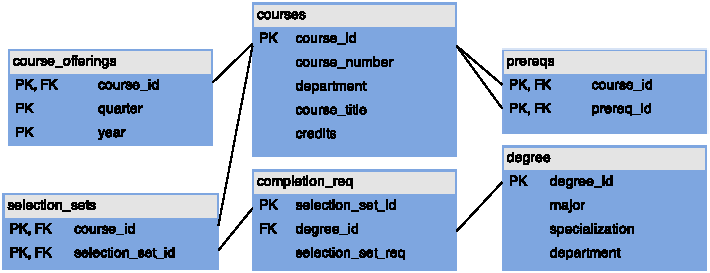
\includegraphics[width=1\textwidth]{CoursePlannerSchema.pdf}\\

In this diagram, boxes relate to database tables that contain the rows of data with the listed columns as attributes. $PK$ indicates an attribute is a $primary key$, which uniquely identifies an entry (or row) of data. $FK$ indicates an attribute is a $foreign key$, which must be a value referencing a primary key in another table. Lines between the table's attributes represent these references (or dependencies). Data that is referenced from other tables as a foreign key cannot be deleted unless that data referenced to it is deleted first. Additionally, adding data with a dependency on another table, requires that the value referencing another table's primary key must be valid. The CourseScheduler handles and enforces both of these constraints through error messages and proper query formulation.
\end{document}